Radiation Survey meters and Contamination Monitors are hand-held ionizing radiation
measuring instruments used to check the radiation level in an environment containing radioactive
sources or radiation-generating equipment. These instruments use gas-filled radiation detectors,
semiconductor radiation detectors, or scintillation detectors. Out of these three, Gas-filled radiation
detectors are very commonly used. Gas-filled detectors have three types: the Ionization chamber, the
Proportional counter, and the Geiger - Muller (G.M.) counter. They all work in their respective voltage
region.
% ----------------------------------------------------------------------
% Instrument 1: G.M Based Instruments
% ----------------------------------------------------------------------
\subsection{G.M Based Instruments (General)}

\subsubsection{Working Principle}
Geiger-Müller (G.M) based instruments operate on the principle of gas ionization in the \textit{Geiger region}.
\begin{itemize}
    \item \textbf{Townsend Avalanche:} The detector consists of a gas-filled tube (usually Argon or Neon with a Halogen quenching agent) with a central anode wire maintained at a high positive potential relative to the cathode wall.
    \item \textbf{Ionization:} When ionizing radiation enters the tube, it creates ion pairs (electrons and positive ions). The strong electric field accelerates electrons toward the anode, causing secondary ionizations.
    \item \textbf{Geiger Discharge:} This results in a massive "avalanche" of electrons (Townsend avalanche) that spreads along the entire length of the anode wire. This produces a large, detectable electrical pulse independent of the energy of the incident radiation.
    \item \textbf{Quenching:} To prevent continuous discharge, a quenching gas (e.g., Chlorine or Bromine) absorbs the energy of positive ions reaching the cathode, stopping the emission of secondary electrons.
\end{itemize}

\subsubsection{Application in Medical Physics}
\begin{itemize}
    \item \textbf{Leakage and Spill Detection:} Used for rapid detection of radioactive spills or leaks in nuclear medicine hot labs.
    \item \textbf{Locating Lost Sources:} Due to their high sensitivity (but low efficiency for gamma), they are ideal for locating lost low-activity seeds (e.g., I-125 seeds in Brachytherapy).
    \item \textbf{General Survey:} Used for "go/no-go" checks to verify if an area is radiation-free.
\end{itemize}



% ----------------------------------------------------------------------
% Instrument 2: Radiation Survey Meter [Model: RM701N]
% ----------------------------------------------------------------------
\subsection{Radiation Survey Meter [Model: RM701N]}

\subsubsection{Working Principle}
The Model RM701N is a microcontroller-based survey meter that utilizes an \textbf{Energy Compensated G.M. Tube} (typically Model GM-130 or equivalent).
\begin{itemize}
    \item \textbf{Energy Compensation:} Unlike standard G.M tubes which over-respond to low-energy gamma rays, this detector is wrapped in a filter (usually tin or lead) to flatten the energy response. This ensures the count rate is proportional to the dose rate across a wide energy range (e.g., 60 keV to 1.25 MeV).
    \item \textbf{Processing:} The instrument counts the pulses from the detector and uses a calibration factor to convert the count rate (CPM) into dose rate units such as mR/hr or $\mu$Sv/hr.
\end{itemize}

\subsubsection{Application in Medical Physics}
\begin{itemize}
    \item \textbf{Area Monitoring:} Routine surveys of corridors and waiting rooms adjacent to radiation therapy bunkers or X-ray suites.
    \item \textbf{Package Inspection:} Checking transport packages (receiving radioactive isotopes) to ensure surface dose rates comply with transport regulations (e.g., Transport Index).
    \item \textbf{Waste Disposal:} Verifying that waste from nuclear medicine patients has decayed to background levels before disposal.
\end{itemize}

\begin{figure}
\centering 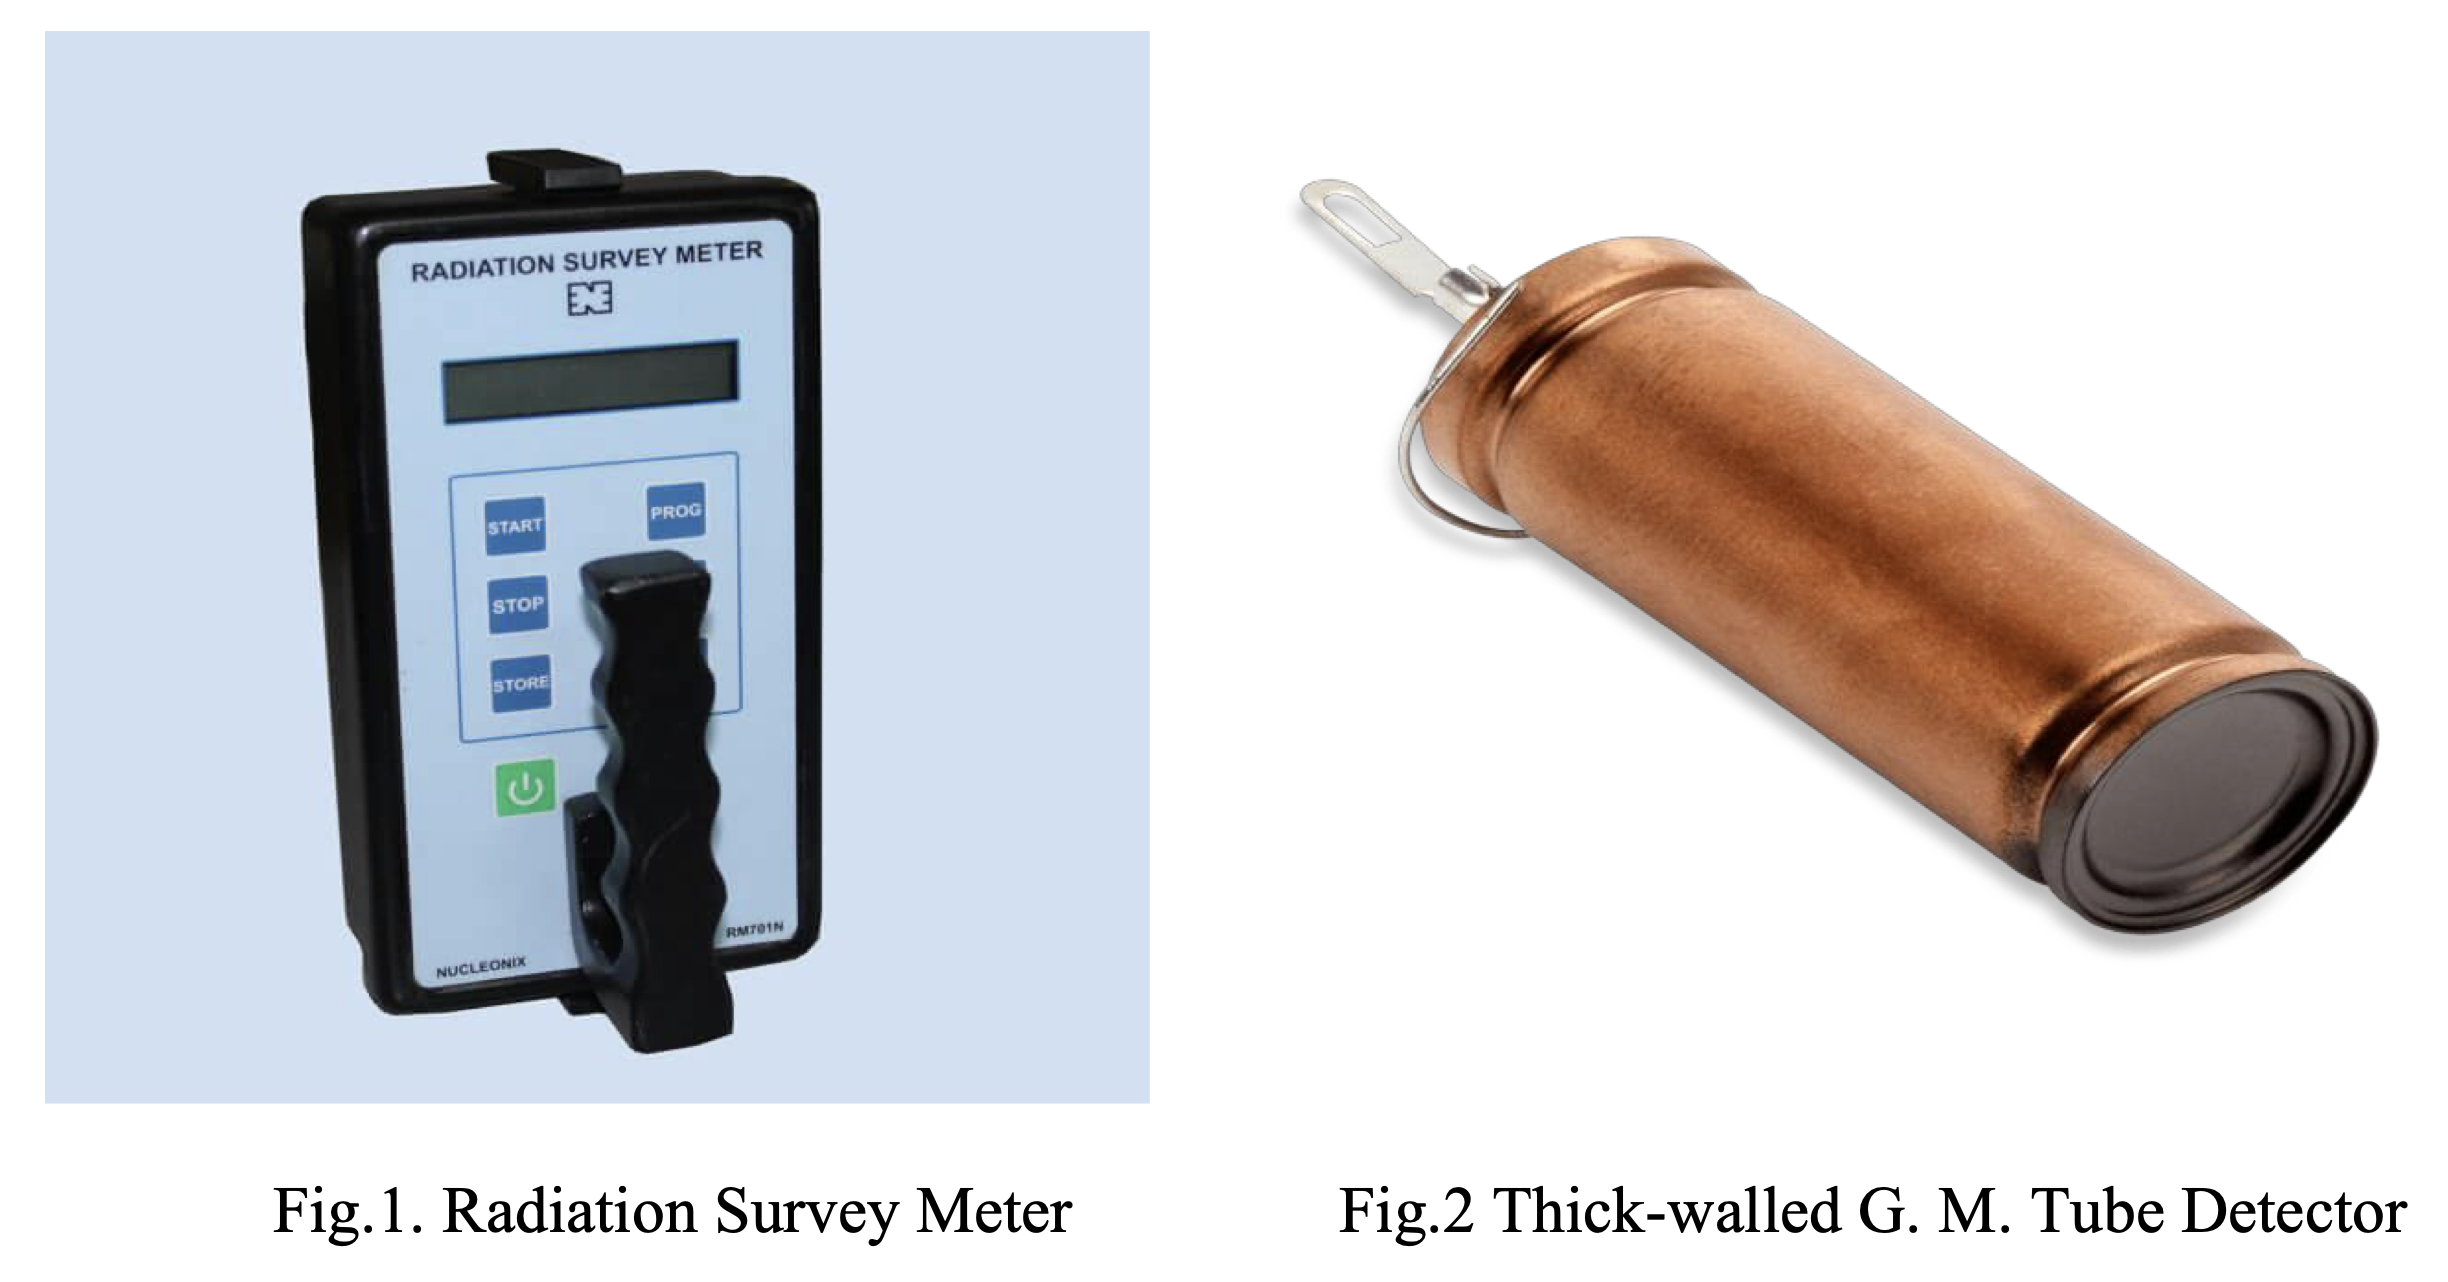
\includegraphics[width=0.7\textwidth]{Figures/TheoryFigure/Instruments1.png}   
\end{figure}

% ----------------------------------------------------------------------
% Instrument 3: Digital Contamination Monitor [Model: CM710N]
% ----------------------------------------------------------------------
\subsection{Digital Contamination Monitor [Model: CM710N]}

\subsubsection{Working Principle}
The CM710N is designed specifically for detecting surface contamination and typically uses a \textbf{Pancake G.M. Probe} (e.g., GM-138).
\begin{itemize}
    \item \textbf{Detector Geometry:} The "pancake" shape provides a large surface area for detection.
    \item \textbf{Thin Window:} It features a very thin mica window ($1.5 - 2.0$ mg/cm$^2$), which allows alpha particles, low-energy beta particles, and gamma rays to enter the detector and cause ionization.
    \item \textbf{Output:} The readout is typically in Counts Per Minute (CPM) or Counts Per Second (CPS), which is directly related to the surface activity (Becquerels) if the efficiency is known.
\end{itemize}

\subsubsection{Application in Medical Physics}
\begin{itemize}
    \item \textbf{Personnel Monitoring:} Checking hands, feet, and clothing of staff leaving the "active" area in Nuclear Medicine.
    \item \textbf{Surface Contamination Checks:} Monitoring workbenches, fume hoods, and floor areas for radioactive contamination (e.g., Tc-99m, I-131).
    \item \textbf{Decontamination Verification:} Confirming that a spill has been successfully cleaned up.
\end{itemize}



% ----------------------------------------------------------------------
% Instrument 4: Micro-digital Pocket Dosimeter [Model: MPD-1501]
% ----------------------------------------------------------------------
\subsection{Micro-digital Pocket Dosimeter [Model: MPD-1501]}

\subsubsection{Working Principle}
The MPD-1501 is an Electronic Personal Dosimeter (EPD) that typically uses a \textbf{Silicon Diode (Semiconductor)} or a miniature energy-compensated G.M. tube.
\begin{itemize}
    \item \textbf{Semiconductor Mode:} Radiation creates electron-hole pairs in the depletion region of the silicon diode. These charges are collected, amplified, and counted.
    \item \textbf{Real-Time Integration:} A microprocessor integrates the pulses over time to calculate the accumulated dose ($\mu$Sv or mrem) and the current dose rate.
    \item \textbf{Alarm Thresholds:} The device has programmable thresholds for dose and dose rate, triggering an audible alarm if limits are exceeded.
\end{itemize}

\subsubsection{Application in Medical Physics}
\begin{itemize}
    \item \textbf{Real-Time Staff Dose Monitoring:} Worn by staff during high-dose procedures (e.g., Interventional Radiology, Brachytherapy loading) to monitor exposure in real-time.
    \item \textbf{ALARA Enforcement:} Helps keeping doses "As Low As Reasonably Achievable" by warning staff immediately when they enter a high-radiation field.
    \item \textbf{Pregnancy Monitoring:} Essential for monitoring the fetal dose of pregnant staff members to ensuring it remains below regulatory limits.
\end{itemize}
\begin{figure}
\centering 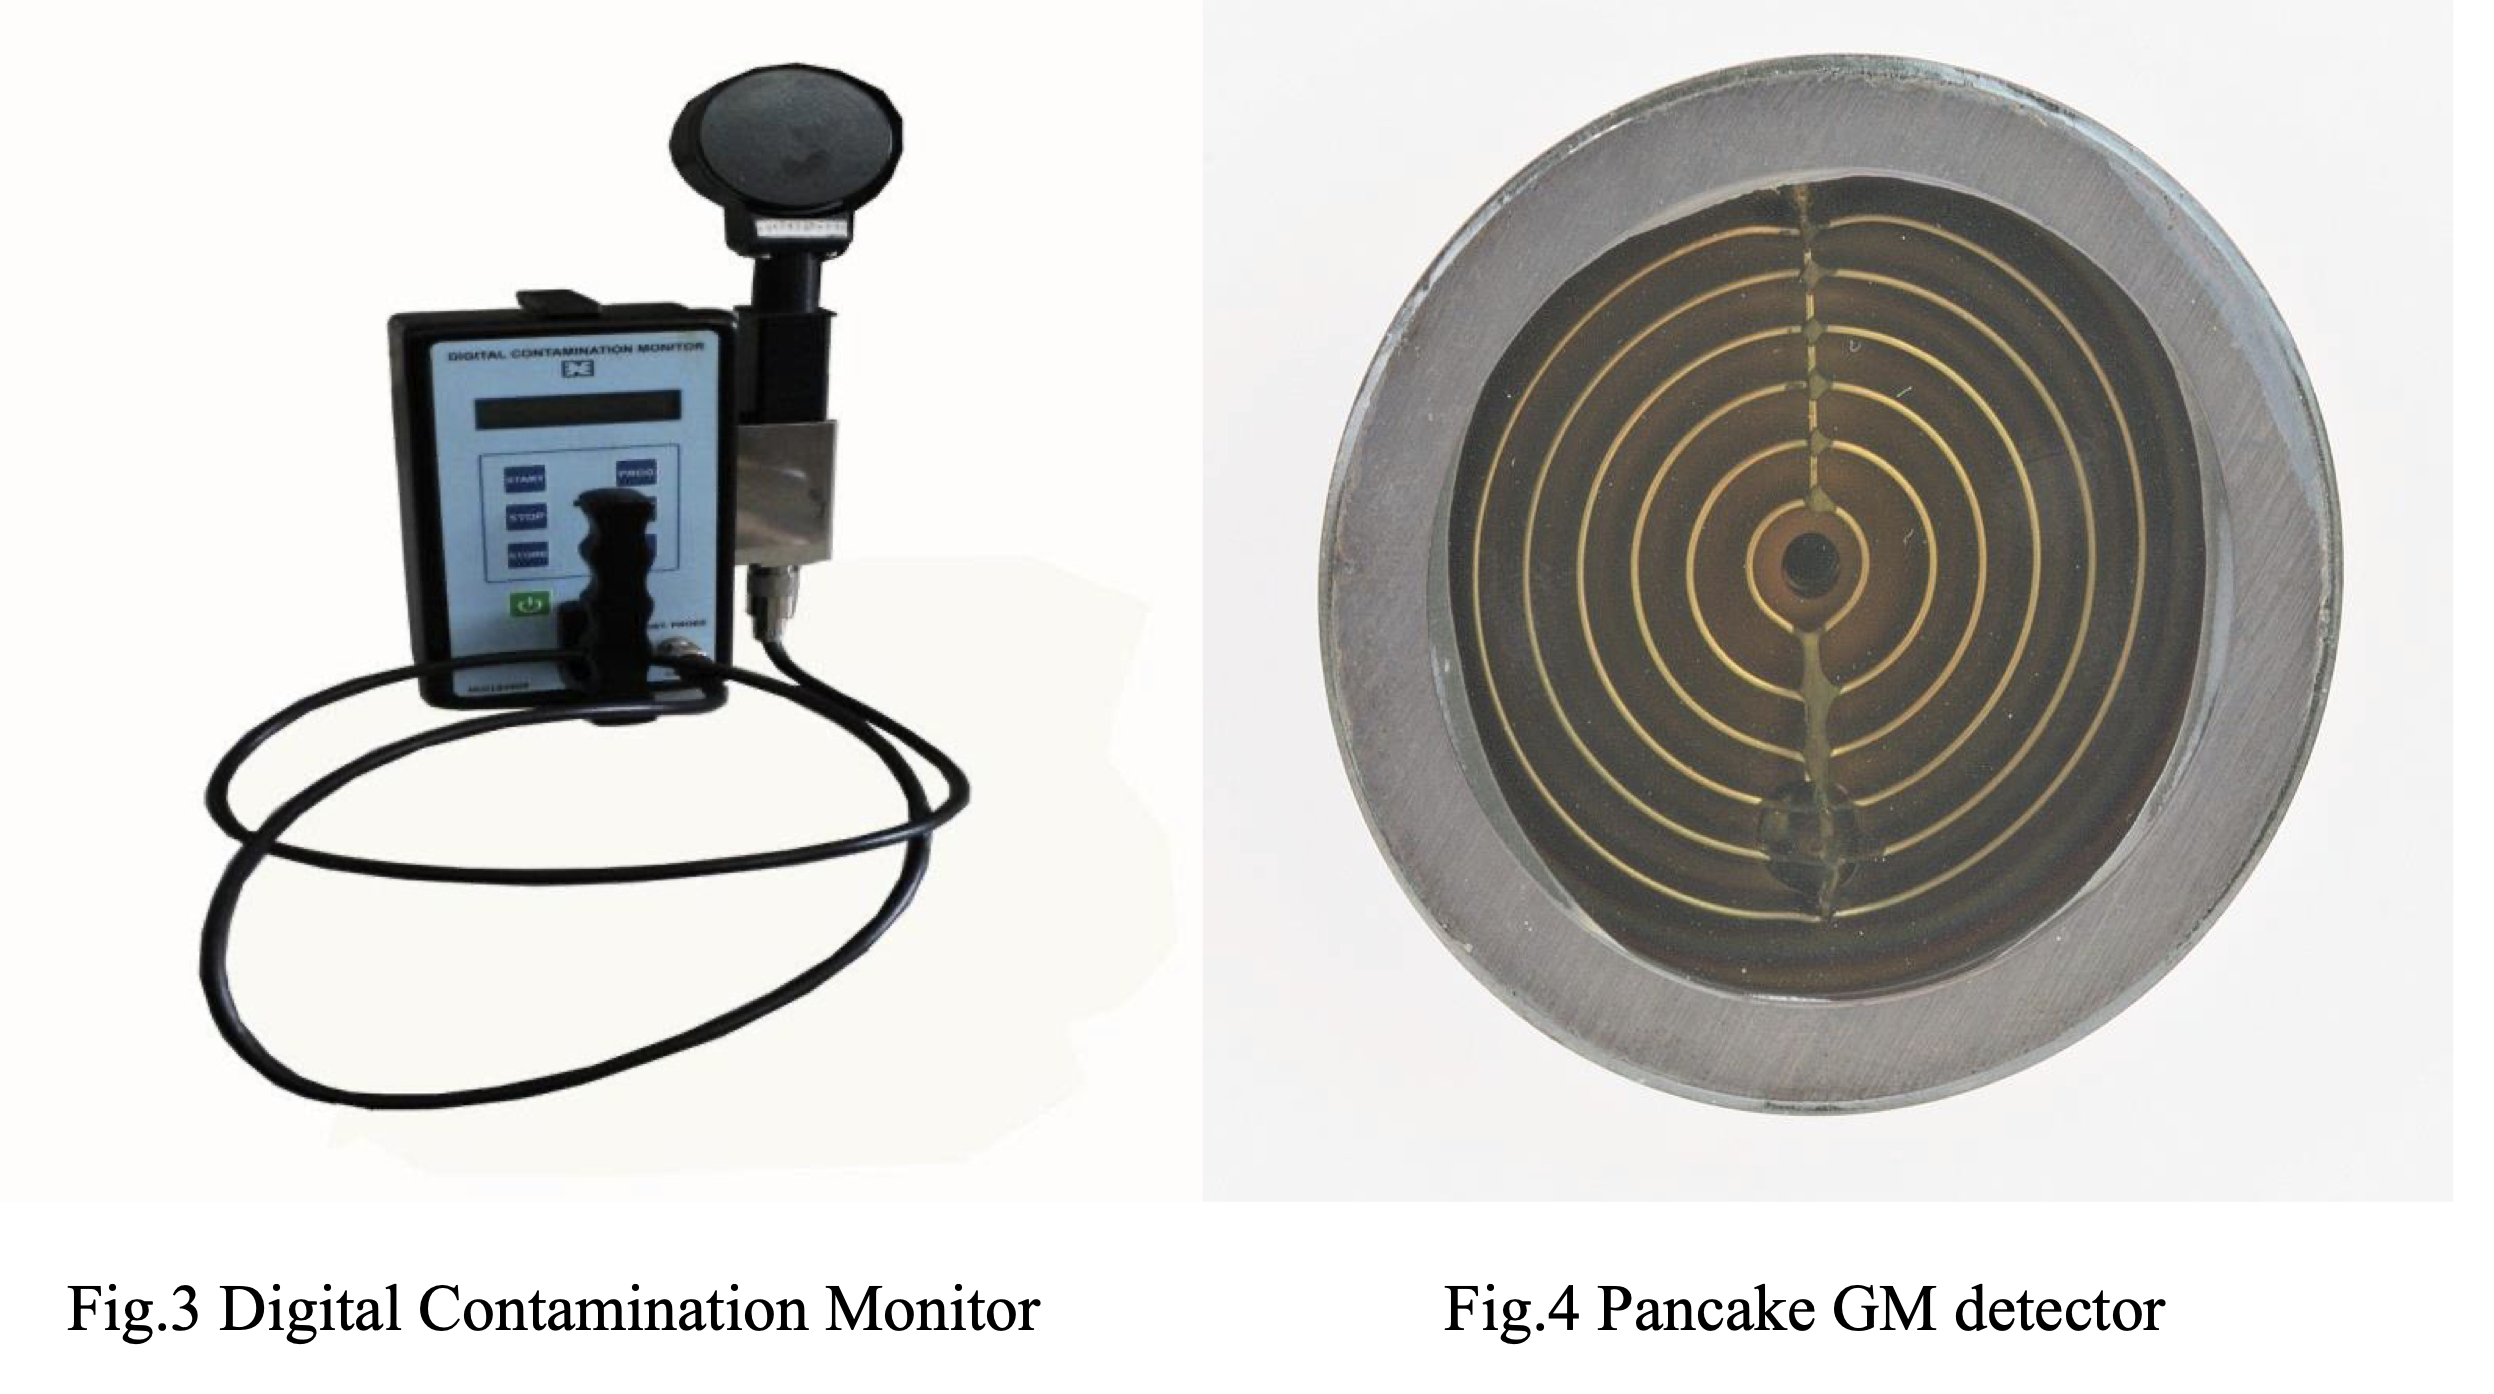
\includegraphics[width=0.7\textwidth]{Figures/TheoryFigure/Instruments2.png}
\end{figure}

% ----------------------------------------------------------------------
% Instrument 5: 451P Pressurized $\mu$R Ion Chamber
% ----------------------------------------------------------------------
\subsection{451P Pressurized $\mu$R Ion Chamber Survey Meter}

\subsubsection{Working Principle}
The 451P is an ionization chamber instrument operating in the \textbf{Ion Saturation Region}.
\begin{itemize}
    \item \textbf{Pressurized Gas:} The chamber is filled with Argon gas pressurized to approximately 8 atmospheres (125 psi).
    \item \textbf{Increased Sensitivity:} The high pressure increases the number of gas molecules, thereby increasing the probability of interaction with ionizing radiation. This allows the measurement of very low exposure rates ($\mu$R/hr).
    \item \textbf{Direct Collection:} Unlike G.M tubes, there is no gas multiplication. The ions produced by radiation are collected directly by the electrodes, creating a tiny current (femtoto-picoamperes) proportional to the energy deposited.
    \item \textbf{Flat Energy Response:} It provides an accurate measurement of exposure (Roentgen) effectively independent of radiation energy (above 25 keV).
\end{itemize}

\subsubsection{Application in Medical Physics}
\begin{itemize}
    \item \textbf{Scatter Surveys:} Measuring scatter radiation levels around CT scanners, Fluoroscopy units, and Linear Accelerators (Linacs) for shielding calculations.
    \item \textbf{Shielding Integrity:} Verifying the thickness and effectiveness of lead lining in X-ray room walls and doors.
    \item \textbf{Linear Accelerator Leakage:} Measuring head leakage radiation from Linacs, where G.M counters would saturate due to the pulsed nature of the beam.
\end{itemize}

\subsection{Calibration of Radiation Instruments}
Calibration is defined as the quantitative determination of a parameter given by a radiation
measuring instrument as a function of the value of the quantity the instrument is intended to measure
under a controlled set of standard conditions. The primary objective of calibration is to ensure that the
instrument is working properly and, hence, can be used for monitoring purposes. Calibration also helps
to find the deviation of the measuring quantity from its actual value, and if needed, the calibration
factor can be adjusted based on the overall measurement accuracy.

All the radiation survey and measuring instruments should be calibrated periodically to ensure
that they are giving correct/valid readings and it is also a regulatory requirement. A convincing method
to calibrate these instruments is to place them in a radiation field of a known dose rate (produced by
radioactive elements) and compare their response with the dose rate. Different calibration factors are
used for $\beta$ and $\gamma$ radiations. The known dose rate can be calculated from the exposure rate constant of
the given radionuclide (Calculation shown below).